\documentclass[dutch, a4paper, 11pt]{article}
\usepackage[utf8]{inputenc}
\usepackage[english]{babel}
\usepackage{pgfplots}
\pgfplotsset{width=10cm,compat=1.9}

%Margins 
\usepackage[a4paper, left=1.27cm,top=1.27cm,right =1.27cm, bottom = 1.4cm]{geometry}

%Load packages
%Algemene packages
\usepackage{babel}
\usepackage{slantsc}
\usepackage{array}
\renewcommand{\arraystretch}{2}
\usepackage{multicol}
\usepackage{multirow}
\usepackage{amsmath}
\usepackage{amsfonts}
\usepackage{booktabs}

%Opsommingen
\usepackage{enumerate}


%Afbeeldingen
\usepackage{graphicx}
\usepackage{wrapfig}

%Gekleurde tekstboxen 
\usepackage[most]{tcolorbox}

%Stop indent
\setlength{\parindent}{0pt}

%Font
\usepackage{cmbright}
\usepackage[OT1]{fontenc}

%Headers and footers
\usepackage{fancyhdr}

\pagestyle{fancy}
\fancyhf{}
\renewcommand{\headrulewidth}{0pt}
\renewcommand{\footrulewidth}{0pt}
\fancyhead[LE,RO]{}
\fancyhead[RE,LO]{}

%Logo in footer
\usepackage{lastpage}
\lfoot{}
\cfoot{\vspace{-5mm} \thepage}
\rfoot{}

%Voorbeeldtekst
\usepackage{lipsum}

%Meerdere kolommen
\usepackage{multicol}
\setlength{\columnsep}{1cm}

%Whitespace na section
\usepackage[compact]{titlesec}  
\titlespacing{\section}{0pt}{2pt}{0pt}

%Tekst kleur
\usepackage{xcolor}

%Nieuwe kleur
%\definecolor{ugent_blue}{rgb}{0.04706, 0.13725, 0.26667}
\definecolor{ugent_blue}{RGB}{30, 100, 200}

%Nummering sections
\renewcommand\thesection{\arabic{section}}
\renewcommand\thesubsection{\thesection.\arabic{subsection}}

%Lay-out hoofdingen
\titleformat*{\section}{\bfseries \normalfont}
\usepackage{sectsty}
\sectionfont{\color{ugent_blue}}
\titlespacing\section{0pt}{10pt plus 4pt minus 4pt}{0pt plus 2pt minus 2pt}

\raggedbottom


%other shit that may be useful
\usepackage{multicol,caption}
\usepackage{mathtools}
\raggedbottom
\newcommand{\HRule}{\hrule}
\abovedisplayskip0pt
\renewcommand{\arraystretch}{1.5}
\newcolumntype{M}[1]{>{\centering\arraybackslash}m{#1}}
\usepackage{lscape}
\newenvironment{Figure}
  {\par\medskip\noindent\minipage{\linewidth}}
  {\endminipage\par\medskip}
\usepackage{float}
\usepackage{hyperref}
\newcommand\myfigure[1]{%
\medskip\noindent\begin{minipage}{\columnwidth}
\centering%
#1%
%figure,caption, and label go here
\end{minipage}\medskip}
\usepackage{caption}
\usepackage{subcaption}
\usepackage{tabularx}
\usepackage{enumerate}
\usepackage{enumitem}

\raggedbottom
\raggedcolumns


\graphicspath{{figures/}}

%units
\newcommand{\MW}{\frac{\text{g}}{\text{mol}}}
\newcommand{\g}{\text{g}}
\newcommand{\ml}{\text{ml}}
\newcommand{\density}{\frac{\text{g}}{\text{ml}}}
\newcommand{\mole}{\text{mol}}
%symbols
\newcommand{\mathtext}[2][]{\text{#2}_{\text{#1}}}

\begin{document}

%Load heading of document
%ugent color
{\color{ugent_blue} \hrule\hrule\hrule}

\vspace*{-0.43mm}
\colorbox{ugent_blue}{\color{white} \bf Report Biomechanics}\\

\noindent\begin{minipage}{0.7\textwidth}% adapt widths of minipages to your needs
{\LARGE \bf \color{ugent_blue} Clinical Movement Analysis Lab Assignment 2022}\\[2mm]

%
{\large Vincent Belpaire}\\
{Supervisor: Prof. Malcolm Forward}\\


{\small University of Ghent}\\
{\small Faculty of Engineering and Architecture}\\
{\small Bachelor of Science: Biomedical Engineering}\\
\end{minipage}%
\hfill%
\begin{minipage}{0.3\textwidth}
\vspace{-2.2cm}
\begin{center}

\includegraphics[width=\linewidth]{ugent_logo}
\end{center}
\end{minipage}\\

\section{Calculations}

    \subsection{Convential radical polymerisation}

    \subsection{ATRP}

    The theoretical molar mass of PMMA is the product of the degree of polymerisation
    with the molar mass of the monomer it consists from, i.e. MMA.
    
    $$\mathtext[PMMA]{MW} = \mathtext[PMMA]{DP} \cdot \mathtext[MMA]{MW} = 50 \cdot 190.65\MW =5006,5\MW$$

    From the formula of degree of polymerisation (there is more than one formula)

    \begin{equation}
        \mathtext[PMMA]{DP} = \frac{\text{\# repeat unit}}{\# polymers},
        \label{eq:DPpmma}
    \end{equation}

    one can derive the amount of initiator needed. Since the number of polymers depends
    on the number of initial radicals present which depends on the number of initiator (I) added
    and the amout of repeat unit is equal to the amout of monomer present one can rewrite the above formula as 

    \begin{equation}
        \# initiator = \frac{\text{\# monomer}}{\mathtext[PMMA]{DP}}.
        \label{eq:numbI}
    \end{equation}

    The amout of monomer present in mol can be derived as

    $$\mathtext[MMA]{m} = 0.943\density\cdot 10\ml = 9.43\g,$$
    $$\mathtext[MMA]{n} = \frac{9.43\g}{100.13\MW} = 9.42\cdot10^{-2}\mole.$$

    Converting formula \ref{eq:numbI} to mol yields

    $$\mathtext[I]{n} = \frac{9.42\cdot10^{-2}\mole}{50}=1.88\cdot10^{-3}\mole.$$

    Multiplying this result with the molecular weight of the initiator gives the
    the amount of initiator needed in grams

    $$\mathtext[I]{m} = 1.88\cdot10^{-3}\mole \cdot 190.65\MW = 3.59\cdot10^{-1}\g.$$

    Now that the amount of initiator is know one can calculate the amount of Cu(I)Br and 
    2,2'-bipyridine [bpy] needed from the know molar ratio [Cu(I)Br][bpy][I] = 1:3:4.

    $$\left\{\begin{matrix}
        \mathtext[Cu(i)Br]{n} = \frac{1}{4}\mathtext[I]{n} = 0.47\cdot10^{-3}\mole,\\
        \mathtext[bpy]{n} = \frac{3}{4}\mathtext[I]{n} = 1.41\cdot10^{-3}\mole.\\
    \end{matrix}\right.$$

    Converting to grams gives

    $$\left\{\begin{matrix}
        \mathtext[Cu(i)Br]{m} = 0.47\mole \cdot 143.45\MW = 67.4 \cdot10^{-3}\g,\\
        \mathtext[bpy]{m} = 1.41\mole \cdot 156.18\MW = 220.2 \cdot10^{-3}\g.\\
    \end{matrix}\right.$$

    At last, the amout of solvent (ethyl acetate) which is present is equimolaire 
    with the amount of MMA present, hence its volume can be calculated as

    $$\mathtext[solvent]{m} = \mathtext[MMA]{n}\cdot 88.11\MW = 8.30\g,$$
    $$\mathtext[solvent]{V} = \frac{\mathtext[solvent]{m}}{0.902\density} = 9.20\ml.$$

\section{Questions}

    \subsection{Reaction steps of the UV-induced radical polymerisation}

    \begin{itemize}
        \item Initiation
                \begin{figure}[H]
                    \centering
                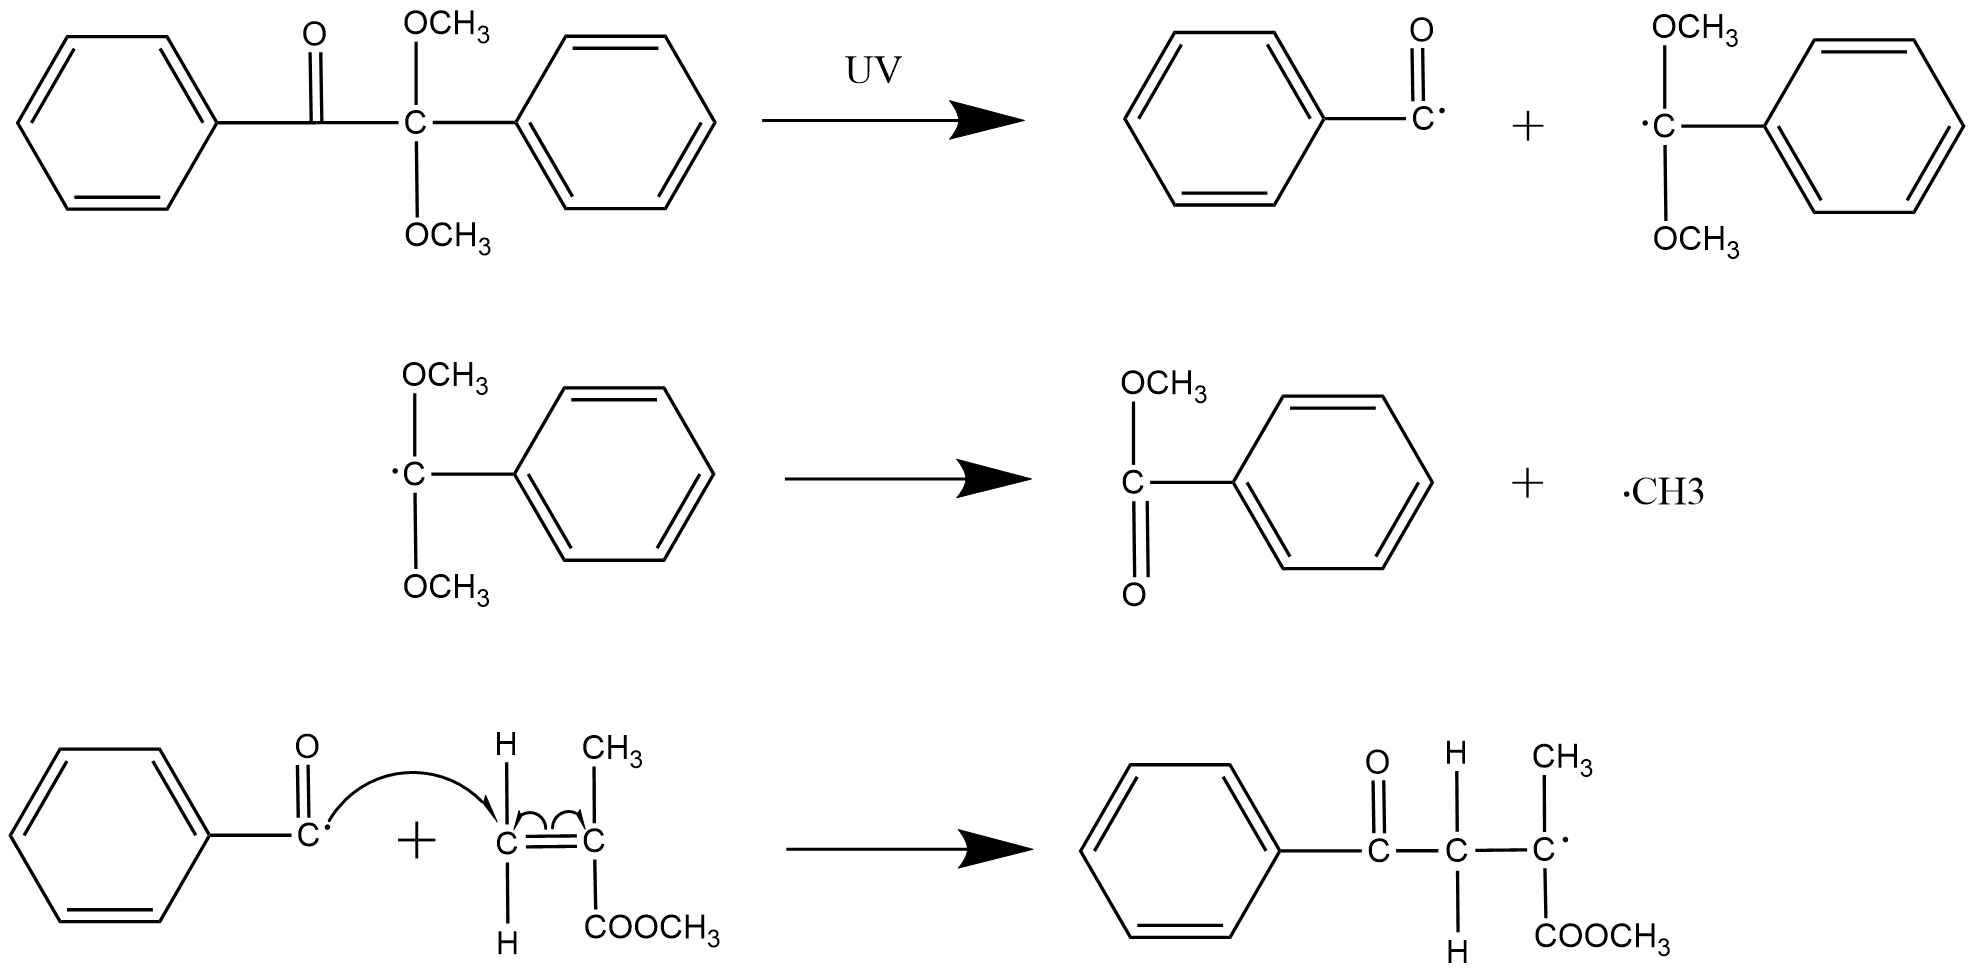
\includegraphics[scale=0.3]{disociatie.png}
                \caption{Initiation}
            \end{figure}
        \item Propagation ($\mathtext[I]{R}$ replaces the initiator radical)
            \begin{figure}[H]
                \centering
                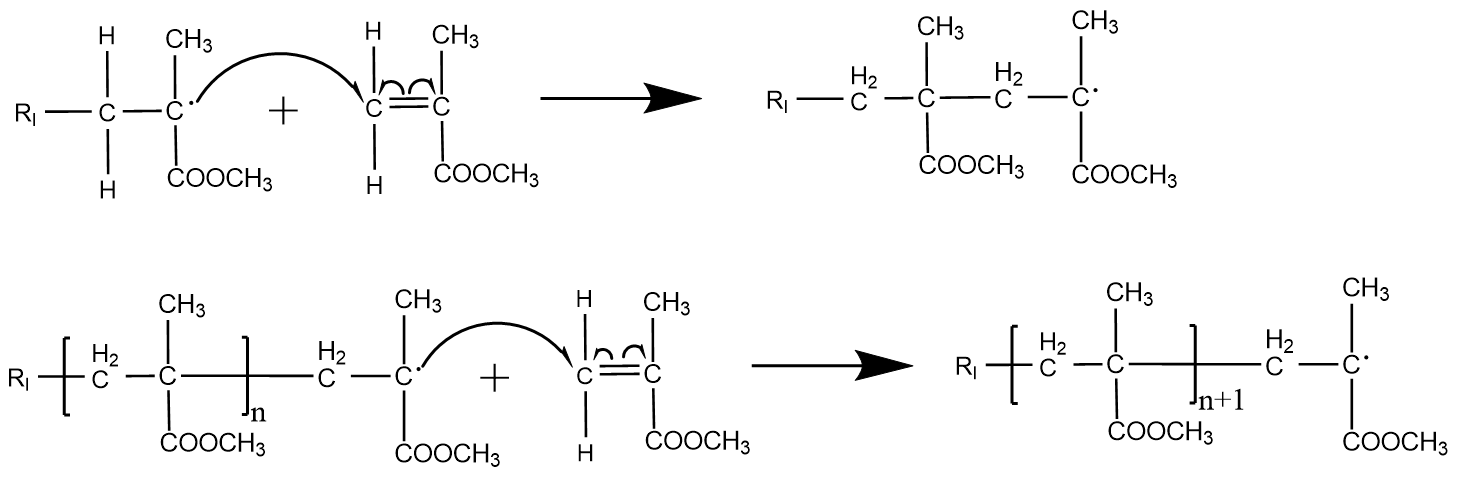
\includegraphics[scale=0.4]{propagation.png}
                \caption{Propagation}
            \end{figure}
        \item Termination (curly string replaces a polymer chain of undefined length)
            \begin{figure}[H]
                \centering
                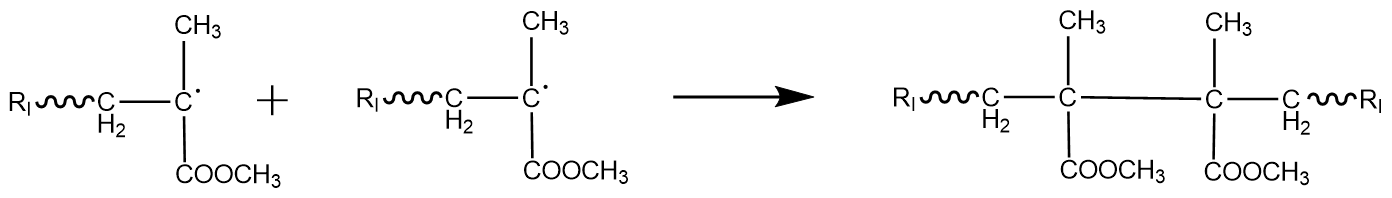
\includegraphics[scale=0.4]{terminatie_combinatie.png}
                \caption{Termination by combination}
            \end{figure}
            \begin{figure}[H]
                \centering
                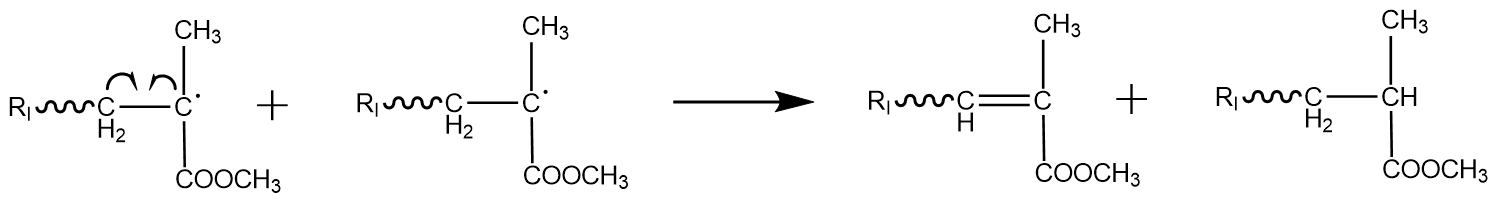
\includegraphics[scale=0.4]{terminatie_disprop.png}
                \caption{Termination by disproportionation}
            \end{figure}
    \end{itemize}

    \subsection{NMR spectroscopy}

Let's denote $\mathrm{I}(x)$ as the integration of a peak at a chemical shift $x$ on the H-NMR-spectra. 
It is know that vinylic protons corresponds to chemical shifts at 5.4 and 6 ppm thus the total amout of 
monomors left is found by the sum $\frac{\mathrm{I}(5.4\text{ppm})+\mathrm{I}(6\text{ppm})}{2}$ (division by two because there are two H-protons present on one vinylic group). The chemical shift corresponding to
the methoxy protons is 3.5 ppm and since the amount of methoxy protons remains the same its integration value $\frac{\mathrm{I}(3.5 \text{ppm})}{3}$  (division by three because there are three H-protons present on one methoxy group)
can be used as a reference of the total amount of monomers present at the start of the reaction. The conversion of the polymerisation reaction 
can then be calculated as

\begin{equation}
    \text{conversion of polymerisation} = 1 - \frac{3}{2}\frac{\mathrm{I}(5.4\text{ppm})+\mathrm{I}(6\text{ppm})}{\mathrm{I}(3.5 \text{ppm})}
    \label{convPoly}
\end{equation}

    \subsection{GPC}

    A higher amount of photo-initiator at the start of the reaction will result in 
    the creation of more polymer chains, hence the average lenght (DP) of one polymer 
    will be lower than the case with lower initial initiator concentrations. Using formula 
    \refeq{eq:DPx} yields the following DP values for the different amout of initiator.

    $$\left\{\begin{matrix}
        \mathtext[1mole\%]{DP} = \frac{100}{1} = 100 \\
        \mathtext[1.5mole\%]{DP} = \frac{100}{1.5} = 66.67 \\
        \mathtext[2mole\%]{DP} = \frac{100}{2} = 50 \\
    \end{matrix}\right.$$

    The polydispersity DPI is calculated as $\frac{\mathtext[w]{M}}{\mathtext[n]{M}}$. For the 
    three different chromatograms one finds the following values

    $$\left\{\begin{matrix}
        \mathtext[GPC1]{DPI} = \frac{67016}{38480} = 1.74\\
        \mathtext[GPC2]{DPI} = \frac{58757}{30089} = 1.95\\
        \mathtext[GPC3]{DPI} = \frac{106029}{38838} = 2.73\\
    \end{matrix}\right.$$

    The DPI value is a measure on the spread of the molecular weight of the polymer. This value is, in most cases, 
    positively correlated with the DP value of the polymer since a higher average chain lenght (higher DP) results 
    in a higher variety on the polymer lenght. Hence high DPI values corresponds to high DP values. Using this correlation 
    results is the following correspondace between the GPC chromatograms and the initial initiator amounts.

    $$\left\{\begin{matrix}
        \text{chromatogram 1} \longleftrightarrow \text{2 mol\%}\\
        \text{chromatogram 2} \longleftrightarrow \text{1.5 mol\%}\\
        \text{chromatogram 3} \longleftrightarrow \text{1 mol\%}\\
    \end{matrix}\right.$$

    \subsection{Similar ATRP experiment}

    The resulting DPI values from the conducted experiment in the video vary between 1.121-1.59. 
    These values are lower the 

    \subsection{Theoretical graph of the molar mass versus conversion}

\end{document}
